\documentclass{article}
\usepackage{../../util/estilo}

\renewcommand{\TituloMain}[0]{Tarea 4}
\newcommand{\MateriaMain}[0]{Implementación de un Algoritmo Genético Paralelo para el Problema del Agente Viajero}
\newcommand{\FechaMain}[0]{23 de Mayo de 2025}

\begin{document}
    \begin{titlepage}
    \begin{centering}

        \thispagestyle{empty}
        
        \setlength{\parindent}{0cm}
        
        \rule{\linewidth}{0.1mm}
        \begin{center}
            \begin{minipage}{2.5cm}
                \begin{center}
                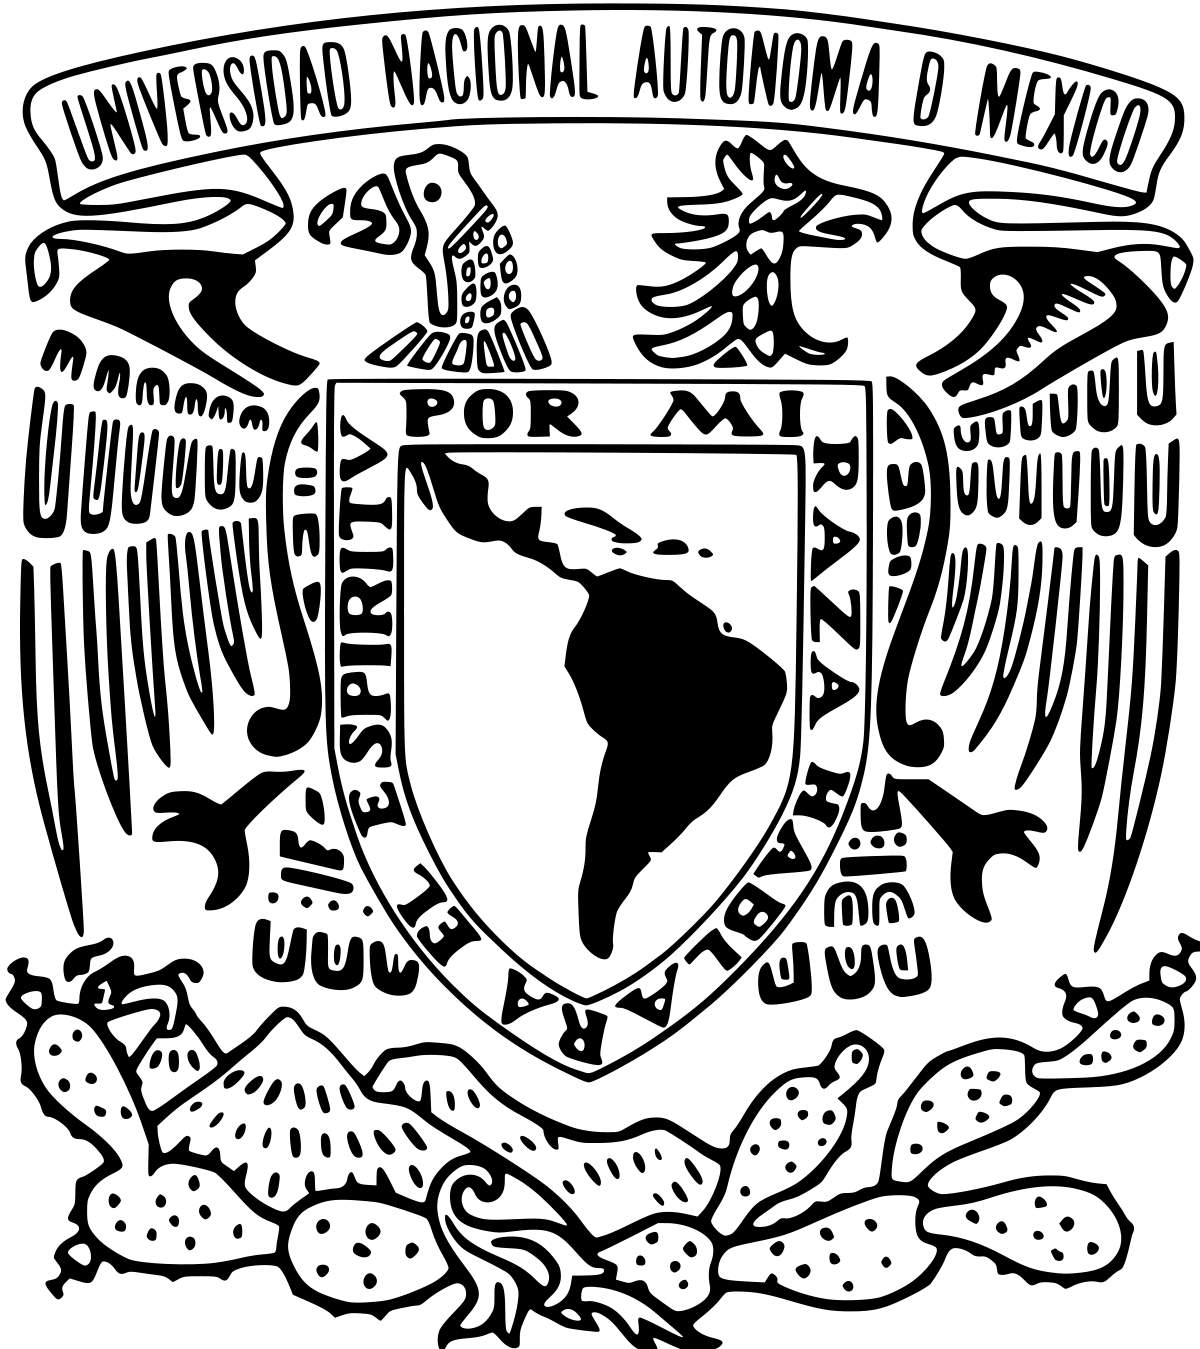
\includegraphics[height=2.7cm]{Logo_UNAM.png}
                \end{center}
            \end{minipage}\hfill
            %--------------
            \begin{minipage}{10cm}
                \begin{center}
                \textbf{ Universidad Nacional Autónoma de México}\\[0.1cm]
                \textbf{Facultad de Ciencias}\\[0.1cm]
                \textbf{\MateriaMain}\\[0.1cm]
                \textbf{Semestre 2025-2}\\[0.1cm]
                \textbf{Integrantes: }\\[0.1cm]
                319526240 - Romero Palacios Santiago\\[0.1cm]
                320268135 - Nava Córdova Mariana\\[0.1cm]
                \FechaMain
                \end{center}
            \end{minipage}\hfill
            %--------------
            \begin{minipage}{2.5cm}
                \begin{center}
                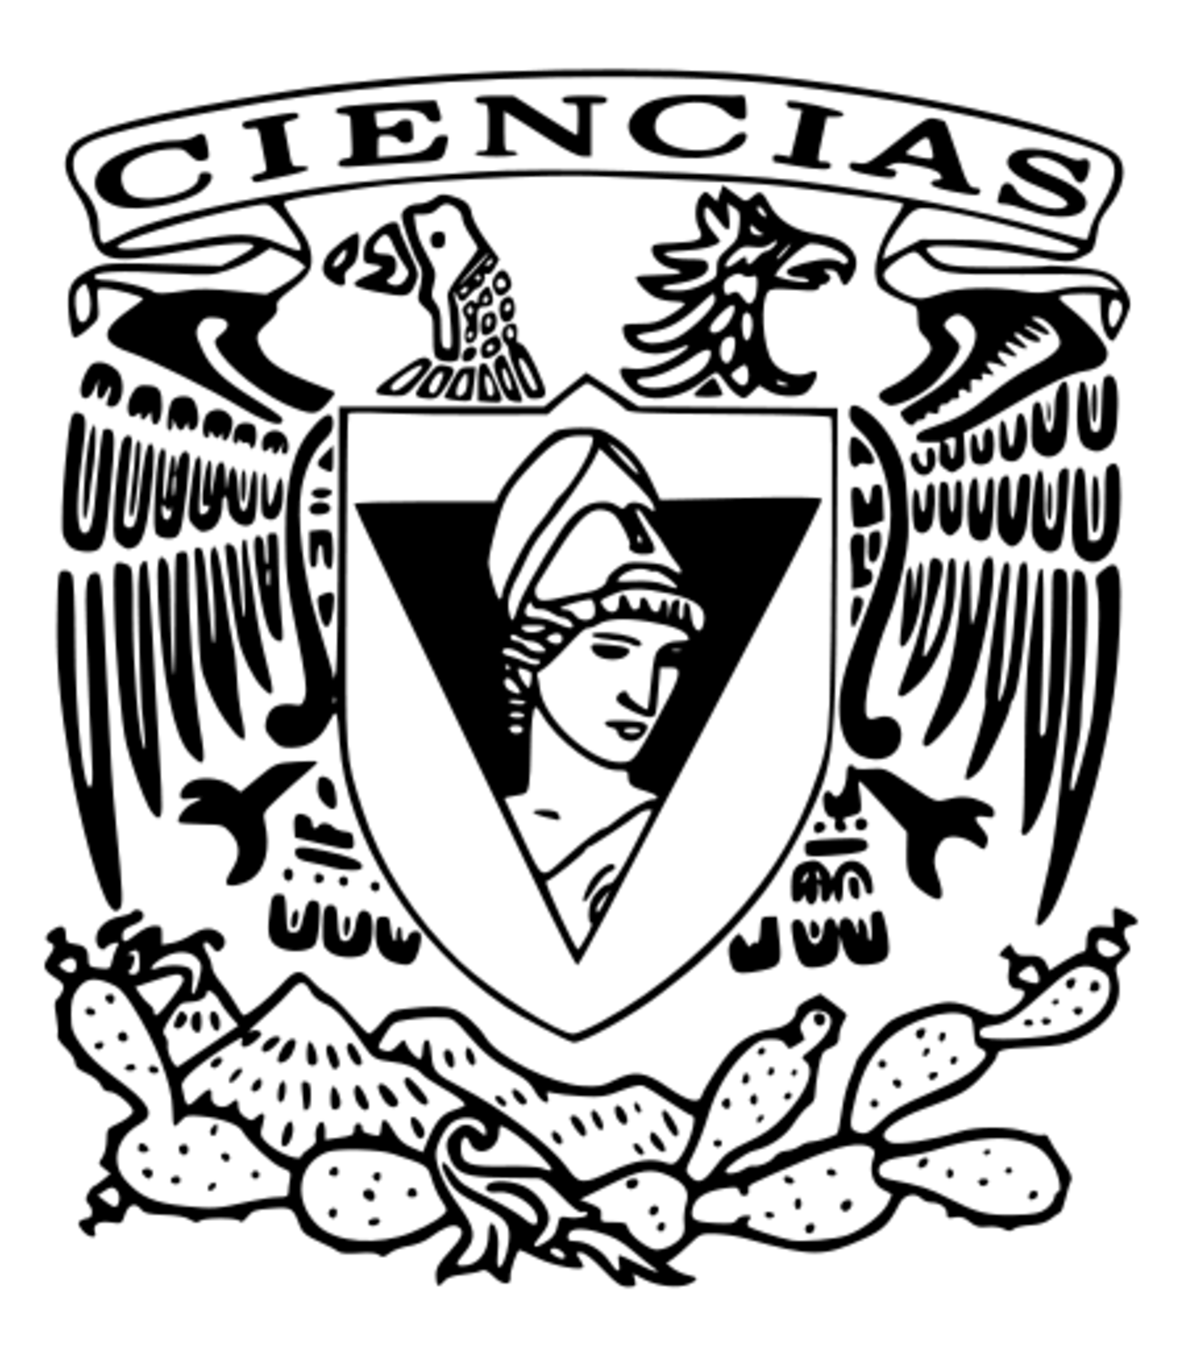
\includegraphics[height=2.7cm]{Logo_FC.png}
                \end{center}
            \end{minipage}
        \end{center}
        \rule{\linewidth}{0.1mm}
        
        
        
        \date{}
        \vspace{0.5cm}
        \vspace{0.5cm}
            {\scshape\Huge \textcolor{RoyalBlue}{\TituloMain} \par}
            {
                \vspace*{2mm}
                \begin{center}\begin{minipage}{6.5cm}
                \centering \tableofcontents
                \end{minipage}\end{center}
            }
        \vspace{0.5cm}
        
        \vspace{1cm}
        \vfill
    \end{centering}
    \end{titlepage}

    %\InsertaSubarchivo{Ejercicio 1}{Ejercicio 1}{1-p_np.tex}

    \pagestyle{logotipos}

    \printbibliography
\end{document}
